\documentclass[14pt]{mmcs_article}
\usepackage[russian]{babel}
\usepackage{amsmath, amsthm, amsfonts, amssymb}

%\graphicspath{{images/}}%путь к рисункам

\begin{document}

%см. РЕКОМЕНДАЦИИ ПО ОФОРМЛЕНИЮ
%И ПРЕДСТАВЛЕНИЮ КУРСОВЫХ И ВЫПУСКНЫХ %КВАЛИФИКАЦИОННЫХ РАБОТ СТУДЕНТОВ ИНСТИТУТА %МАТЕМАТИКИ, МЕХАНИКИ И КОМПЬЮТЕРНЫХ НАУК


% ----------------------------------
% Внимание!
% Изменяйте только строки, перед которыми стоят знаки комментариев
% ----------------------------------

\thispagestyle{empty}
\begin{singlespacing}
\begin{center}

МИНОБРНАУКИ РОССИИ\\ [12pt]
Федеральное государственное автономное образовательное\\
учреждение высшего образования\\
<<Южный федеральный университет>>

\vspace{\baselineskip}
Институт математики, механики\\
и компьютерных наук им.~И.\,И.~Воровича

\vspace{\baselineskip}
% Название выпускающей кафедры
Кафедра алгебры и дискретной математики

\vfill
% Фамилия Имя Отчество студента
\textbf{Иванов Иван Сергеевич}

\vspace{\baselineskip}
%НАЗВАНИЕ РАБОТЫ должно полностью соответствовать
% приказу по ЮФУ (для выпускных квалификационных работ)
{\bf НАЗВАНИЕ РАБОТЫ, \\
РАЗБИТОЕ ПРИ НЕОБХОДИМОСТИ \\
НА НЕСКОЛЬКО СТРОК }

\vspace{15mm}
ВЫПУСКНАЯ КВАЛИФИКАЦИОННАЯ РАБОТА\\
по направлению подготовки\\
% Направление обучения
% раскомментируйте нужную строчку
02.03.02~-- Фундаментальная информатика и информационные технологии
% 01.03.01~-- Математика
% 01.03.02~-- Прикладная математика и информатика
% 01.03.03~-- Механика и математическое моделирование 	


\vspace{10mm}
\textbf{Научный руководитель~--}\\
% указать данные о руководителе
% должность, степень, звание Фамилия Имя Отчество
проф., д.\,ф.-м.\,н. Сергеев Петр Сергеевич

\vspace{15mm}

\noindent
% указать Фамилию и инициалы 
% заведующего выпускающей кафедры
\begin{flushleft}
Допущено к защите:\\
заведующий кафедрой \underline{\hspace*{65mm}} Сидоров С.\,С.
\end{flushleft}




\vfill
% год!
Ростов-на-Дону -- 2020

\end{center}

\singlespacing
\end{singlespacing} 

\renewcommand{\contentsname}{Оглавление}

\tableofcontents

%=======================
\newpage
\addcontentsline{toc}{section}{Постановка задачи}

\section*{Постановка задачи}

%=======================
\newpage
\addcontentsline{toc}{section}{Введение}
\section*{Введение}

В описании современных стандартов передачи данных много внимания уделено контролю за ошибками, неизбежно возникающими в любом канале связи. В теории кодирования применяют много различных подходов к проблеме коррекции подобных ошибок. Обычно для этого вместе с последовательностью данных передают последовательность проверочных битов, которые позволяют обнаружить и даже исправить ошибочно переданные сигналы. Примером таких алгоритмов могут служить коды с малой плотностью проверок на чётность \cite{johnson}.

Каждому проверочному биту соответствует набор информационных битов, в соответствии с которыми вычисляется его значение. От того, как задано это соотношение, сильно зависит эффективность процесса передачи данных, поэтому целесообразно искать алгоритмы, максимально эффективно соотносящие поток информации с данными для проверки.

Методы построения таких соотношений, используемые в крупных компаниях, попадают под соглашения о неразглашении, Однако известны такие методы, как перебор возможных матриц \cite{bruteforce} и псевдослучайные пермутации матриц \cite{permutations}.

Далее мы рассмотрим подходы к решению данной задачи, основанные на анализе графов с определённой структурой.

%=======================
\newpage
\section{Основные понятия и утверждения}\label{dsfs}

\textbf{Определение 1.}

\textsl{Графом Таннера} будем называть двудольный неориентированный граф.

Вершины из одной доли графа Таннера соответствуют информационным битам, а вершины из другой ~--- проверочным. Вершины из этих долей называют \textsl{информационными} и \textsl{проверочными} соответственно. Рёбра же определяют взаимосвязь между этими двумя потоками данных.

\textbf{Определение 2.}

\textsl{Обхватом графа} называют длину его минимального цикла.

Отметим, что обхват любого графа Таннера является чётным.

Известно, что на практике для кодирования эффективнее использовать графы с большим обхватом.

\textbf{Определение 3.}

Граф Таннера называется \textsl{(m, n)-регулярным}, если степень каждой проверочной вершины равна m, а степень каждой информационной вершины равна n.

\textbf{Определение 4.}

Будем называть граф Таннера \textsl{почти (3, n)-регулярным}, если большая часть информационных вершин имеет степень 3, а степень остальных не меньше двух.

На практике обычно используют (3, n)-регулярные или почти (3, n)-регулярные графы.

%=======================
\newpage
\section{Графы с регулярной структурой}

\subsection{Определение}

Графом с регулярной структурой, будем называть двудольный граф, который сотоит из заданного количества одинаковых компонент, между которыми строятся дуги таким образом, что граф изоморфен сам себе по отображению, циклически смещающему все вершины $i$-той компоненты в аналогичные вершины $i + 1 \pmod K$-той компоненты, где $K$ ~--- общее количество компонент в графе.

Граф с регулярной структурой задаётся четвёркой $\langle c, i, K \in \mathbb{N}, f: \mathbb{Z} \rightarrow \{ \mathbb{Z} \times \mathbb{N} \} \rangle$, где $c$ ~--- это количество проверочных вершин в компоненте, $i$ ~--- количество информационных вершин в компоненте, $K$ ~--- количество компонент, а $f$ ~--- отображение, по которому строятся дуги. Оно сопоставляет номера проверочных вершины внутри компоненты в относительные номера компонент и номера информационных вершин внутри компонент, с которыми связана дуга.

На рис. \ref{stud:fig:1} изображён граф с регулярными структурами, заданный четвёркой $\langle 1, 2, 4, f: f(1) = \{ (0, 1), (0, 2), (-1, 2), (1, 1) \} \rangle$

\begin{figure}[H]
  \centering
  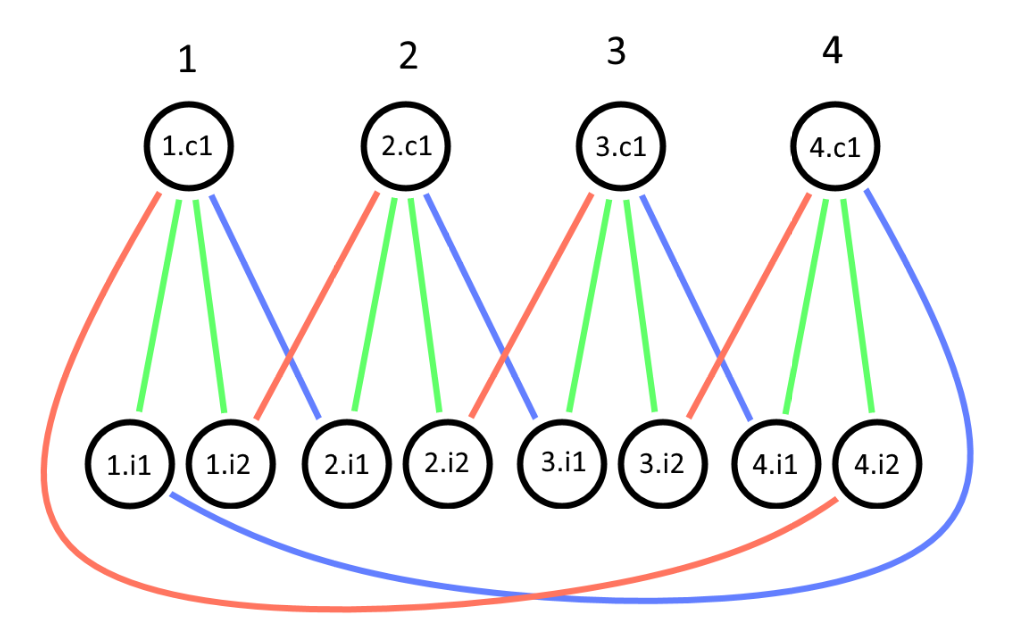
\includegraphics[scale=0.4]{Fig_1.png}
  \caption{ Граф с регулярной структурой. Компоненты пронумерованы от 1 до 4. Вершины помечены в формате \{номер компонетны\}.\{i, если вершина информационная, с, если проверочная\}\{номер вершины\} }\label{stud:fig:1}
\end{figure}

При анализе таких графов можно опустить параметр $K$, считая его достаточно большим, а затем при использовании подобрать его исходя из практических требований к размеру графа. Поэтому далее будем говорить о том, что регулярный граф задаётся тройкой $\langle c, i, f \rangle$.

\subsection{Представление графов с регулярной структурой}

Тройку $\langle c, i, f \rangle$, которой задаётся граф с регулярной структурой, можно наглядно изобразить в виде компоненты, в которой проведены дуги проведены в соответствующие информационные вершины в этой же самой компоненте. Дуги следует пометить относительным номером компоненты, с которой она связана.

На рис. \ref{stud:fig:2} изображено подобное представление графа, соответствующего тройке $\langle 1, 2, f: f(1) = \{ (0, 1), (0, 2), (-1, 2), (1, 1) \} \rangle$

\begin{figure}[H]
  \centering
  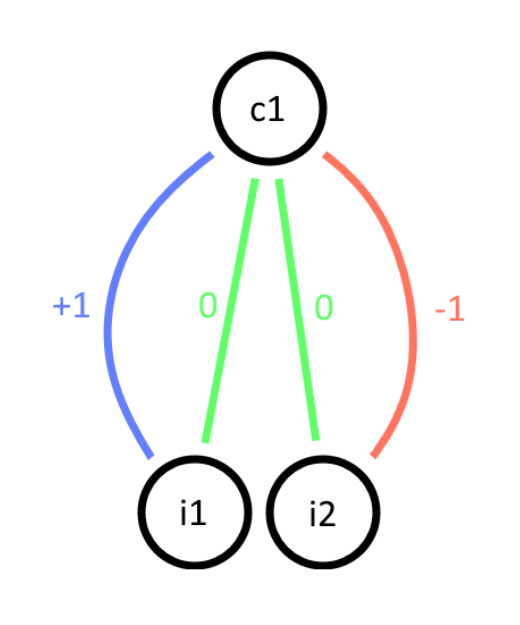
\includegraphics[scale=0.4]{Fig_2.png}
  \caption{ Упрощённое представление графа с регулярной структурой. }
  \label{stud:fig:2}
\end{figure}

\subsection{Поиск циклов в графах с регулярной структурой}

Так как основная задача при построении таких графов ~--- контроллировать длину минимального цикла, рассмотрим алгоритм поиска циклов в графе с регулярной структурой, заданном тройкой $\langle c, i, f \rangle$.

\textbf{Лемма 1.}

Если в графе с регулярными структурами есть цикл длины $t$, то через одну из проверочных вершин первой компоненты проходит цикл длины $t$.

\textbf{Доказательство.}

Любой цикл в двудольном графе проходит через какую-то проверочную вершину. Обозначим номер компоненты $d$, а индекс проверочной вершины внутри компоненты через $j$. Из определения графа с регулярными компонентами, следует, что он изоморфен сам себе по отображению, циклически сдвигающему все вершины каждой $i$-той компоненты в $i - d \pmod K$-тую компоненту. Следовательно, существует цикл длины $t$, проходящий через $j$-тую проверочную вершину первой компоненты.

\qed

Из леммы 1 следует, что чтобы показать, что минимальный цикл в графе имеет длину $t$, достаточно убедиться, что через проверочные вершины одной компоненты не проходят циклы короче, чем $t$.

\textbf{Алгоритм 1.} 

В листинге \ref{stud:lst:1} приведён алгоритм поиска циклов проходящих через $j$-тую проверочную вершину. Для того, чтобы найти кратчайший цикл во всём графе нужно применить алгоритм ко всем проверочным вершинам компоненты.

\textbf{Теорема 1.}

Приведённый алгоритм находит кратчайший цикл, проходящий через заданную проверочную вершину.

\textbf{Доказательство.}

Если вершина в неком поколении $\phi$ помечена неким числом $n$, значит кратчайший путь до этой вершины в компоненте $n$ от заданной проверочной вершины равен $\phi$, так как фактически осуществляется поиск в ширину, который находит кратчайшие пути. Если существует два кратчайших пути длмны $\phi$ без общих вершин (кроме начальной и конечной) до вершины, алгоритм завершается.

Если существует кратчайший цикл длины $t$, значит в этом цикле есть вершина $v$, до которой существует два пути длины $t / 2$, в которых нет совпадающий вершин. Так как цикл кратчайший, то пути до вершины $v$ короче, чем $t / 2$ нет. Если есть два пути длины $t / 2$, у которых есть общие вершины (кроме начальной и конечной), то они образуют цикл длины, меньшей, чем $t$, следовательно таких путей нет.

Таким образом, алгоритм обязательно найдёт кратчайший цикл.

\qed

\begin{lstlisting}[caption={Алгоритм поиска циклов}, label=stud:lst:1]
//   Возвращает длину самого короткого цикла, проходящего через j- тую
// проверочную вершину компоненты или -1, если циклов меньше или равных
// max-cycle не найдено
fn find-cycle(j, max-cycle) {
    // Начинаем работу с нулевого поколения
    generation = 0;
    //   Словарь где ключами выступают вершины и поколения,
    // а значения - множества меток.
    //   Метки соответствуют пройденному пути.
    //   Изначально j- тая проверочная вершина помечена нулём.
    labels = { (control(j), generation): { 0 } };
    повторять, пока generation >= max-cycle / 2 { 
        для всех вершин vertex в текущем поколении {
            generation += 1;
            для всех дуг edge, соединённых с vertex {
                для всех меток label на вершине vertex
                в текущем поколении {
                    next-vertex = вершина, с которой соединена дуга;
                    //   Если проходим по дуге снизу-вверх,
                    // берём сдвиг с обратным знаком
                    shift=edge.label*(vertex проверочная ?1:-1);
                    shifted-label = label + shift;

                    если next-vertex уже помечена shifted-label
                    в одном из предыдущих поколений поколении:
                        continue;

                    если next-vertex уже помечена shifted-label 
                    в текущем поколении:
                        return generation * 2;

                    пометить next-vertex shifted-label
                    в текущем поколении
                }
            }
        }
    }
    return -1;
}
\end{lstlisting}

На рис. \ref{stud:fig:3} изображён пример работы алгоритма. Для удобства поколения пометок обозначены цветами. Нулевое поколение ~--- синим, первое ~--- зелёным, второе ~--- голубым, третье ~--- розовым, четвёртое ~--- жёлтым. Совпадающие метки в четвёртом поколении обведены красными рамками. Алгоритм легко доработать так, чтобы он возвращао список вершин, из которых состоит цикл. Для этого следует к пометкам добавить ссылку на родительскую вершину и затем, когда цикл найден, вернуться по ссылкам назад, собирая список вершин. На рис. \ref{stud:fig:4} изображён один из циклов, найденных в результате работы алгоритма. 

\begin{figure}[H]
  \centering
  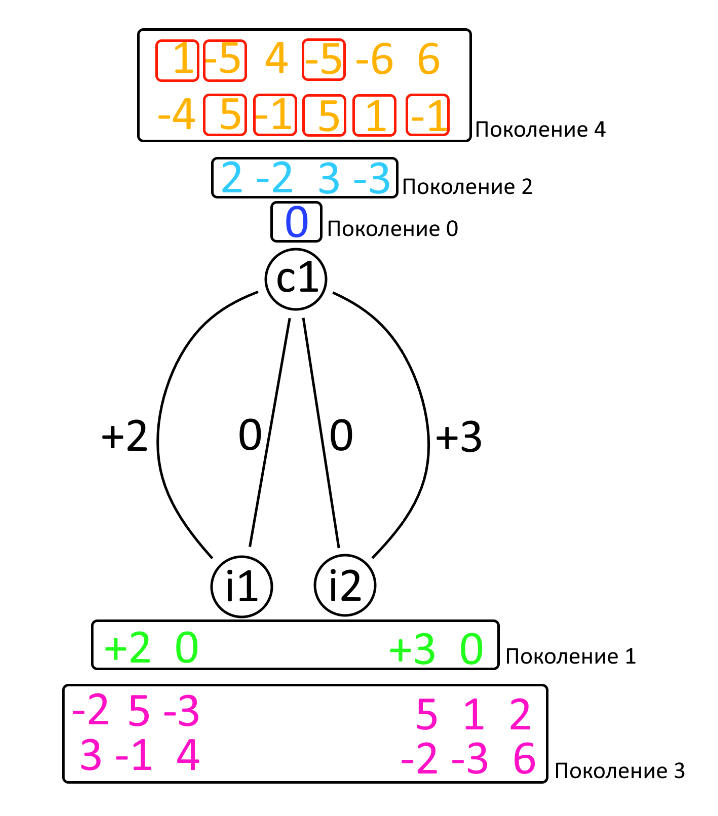
\includegraphics[scale=0.6]{Fig_3.png}
  \caption{ Пример работы алгоритма поиска циклов. }
  \label{stud:fig:3}
\end{figure}

\begin{figure}[H]
  \centering
  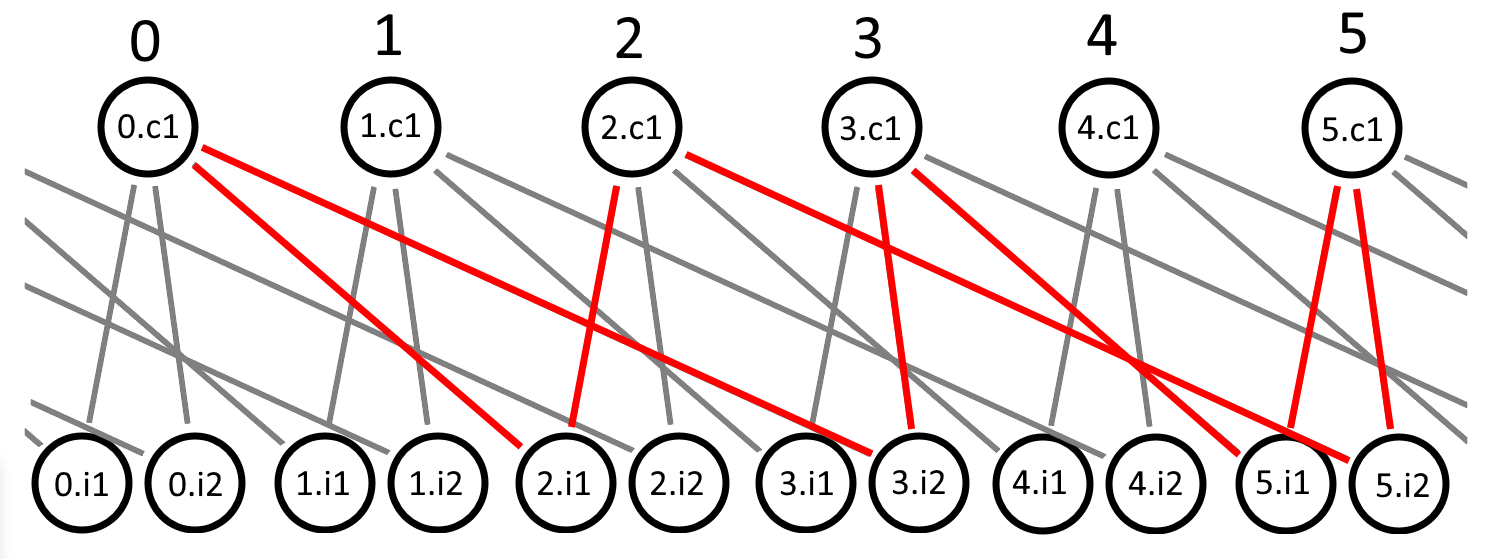
\includegraphics[scale=0.4]{Fig_4.png}
  \caption{ Пример цикла, найденного алгоритмом поиска циклов. }
  \label{stud:fig:4}
\end{figure}

На рис. \ref{stud:fig:5} изображён пример работы алгоритма на графе, дуги которого имеют неизвестные сдвиги, обозначенные буквами $a$, $b$ и $c$. Видно, что вне зависимости от значений переменных найден цикл-шестёрка.

\textbf{Замечание.}

(3,n)-регулярные графы с регулярными структурами и обхватом больше шести нельзя построить, если в компоненте только одна проверочная вершина, так как всякий такой граф будет содержать циклы-шестёрки, проходящие через первую информационную вершину.
 
\begin{figure}[H]
  \centering
  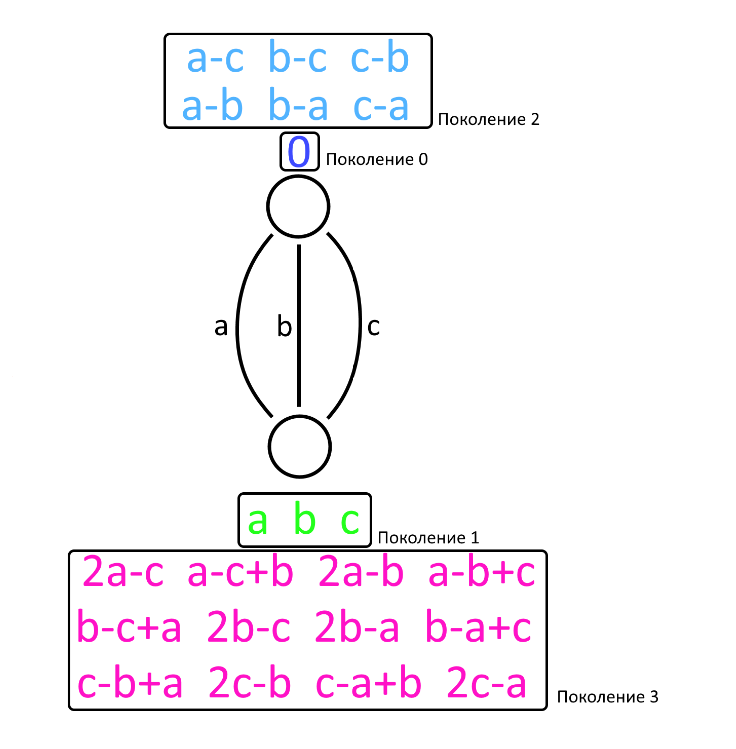
\includegraphics[scale=0.6]{Fig_5.png}
  \caption{ Пример поиска цикла на графе с неизвестными сдвигами. }
  \label{stud:fig:5}
\end{figure}
   
%=======================
\newpage

\section{Построение графа с заданным минимальным циклом.}

\textbf{Алгоритм 2.}

Для того, чтобы построить граф с заданным обхватом $t$, обозначим сдвиги на дугах как $x_1$, $x_2$, ..., $x_e$. Сделаем $t/2$ итераций алгоритма поиска циклов. Если алгоритм нашёл цикл, то выбранная структура компоненты не позволяет построить граф с заданным обхватом, необходимо увеличить количенство проверочных вершин.

Множество всех меток, полученных в результате работы алгоритма, разделяем по поколению и вершине на подмножества $U(v, d)$, где $v$ пробегает множество вершин, а $d$ ~--- множество поколений. По полученным подмножествам составляем систему неравенств вида $U(v, d)[i] \neq U(v,d)[j] \forall i \neq j; v; d$.

Находим решение полученной системы неравенств, строим граф со сдвигами дуг равными значениям полученного решения. В данном графе размер минимального цикла будет больше или равен $t$. 

\textbf{Теорема.}

В результате карректного завершения работы алгоритма 2 получается граф с обхватом больше или равным требуемому.

\textbf{Доказательство.}

Допустим, мы нашли решение системы неравенств, равное $(\alpha_1, \alpha_2, ..., \alpha_e)$. Построим граф по этому решению. Делаем $t/2$ итераций алгоритма поиска циклов. Так как система неравенств гарантирует, что метки в одной вершине и одном поколении отличаются, алгоритм не завершается. Следовательно обхват графа больше или равен $t$.

\qed

\textbf{Замечание.}

При использовании алгоритма 2 удобно в качестве пометок использовать вместо сумм вида $a_1 x_1 + a_2 x_2 + ... + a_e x_e$ кортежи вида $(a_1, a_2, ..., a_e)$. Неравенство вида $a_1 x_1 + ... + z_e x_e \neq b_1 x_1 + ... + b_e x_e$ можно записывать в виде кортежа $(a_1 - b_1, ..., a_e - b_e)$. Такой кортеж можно домножать на константу, что эквивалентно домножению на константу обеих сторон неравенства. 

\begin{figure}[H]
  \centering
  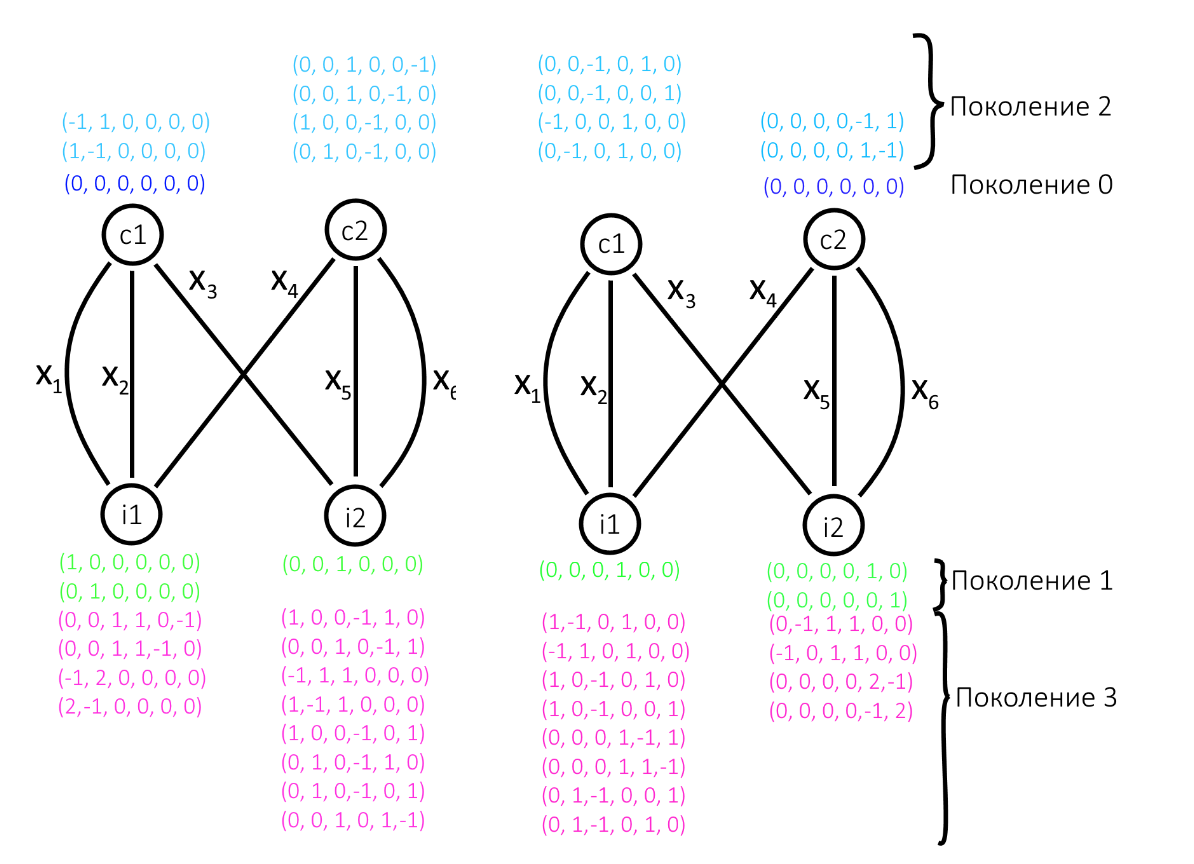
\includegraphics[scale=0.5]{Fig_6.png}
  \caption{ Первый этап работе алгоритма 2. }
  \label{stud:fig:6}
\end{figure}

На рис. \ref{stud:fig:6} изображён первый этап работы алгоритма 2 для графа с регулярными структурами, заданного тройкой $ \langle 2; 2; f\rangle $, где $ f(1) = \{ (x1, 1),\\ (x2, 1), (x3, 2) \} $, а $f(2) = \{ (x4, 1), (x5, 2), (x6, 2) \}$. Выполняется четыре итерации поиска циклов в общем виде для первой и второй проверочных вершин. Алгоритм не нашёл одинаковых кортежей в множествах пометок с одинаковой вершиной и поколением, значит, есть смысл составлять систему неравенств и искать её решение.

Система неравенств (\ref{stud:eqs:1}) построена из множеств меток, полученных в результате работы первого этапа алгоритма. Неравенства упрощены, повторения убраны.

\begin{equation}
  \centering
    \left\{
      \begin{array}{ll}
        (1,-1,\ \ 0,\ \ 0,\ \ 0,\ \ 0)\\
        (0,\ \ 1,-1,-1,\ \ 0,\ \ 1)\\
        (0,\ \ 1,-1,-1,\ \ 1,\ \ 0)\\
        (1,\ \ 0,-1,-1,\ \ 0,\ \ 1)\\
        (1,\ \ 0,-1,-1,\ \ 1,\ \ 0)\\
        (0,\ \ 0,\ \ 0,\ \ 0,\ \ 1,-1)\\
        (1,\ \ 0,-1,-1,-1,\ \ 2)\\
        (1,-1,\ \ 0,\ \ 0,-1,\ \ 1)\\
        (2,-1,-1,-1,\ \ 0,\ \ 1)\\
        (1,-1,\ \ 0,\ \ 0,\ \ 1,-1)\\
        (2,-1,-1,-1,\ \ 1,\ \ 0)\\
        (1,\ \ 0,-1,-1,\ \ 2,-1)\\
        (0,\ \ 1,-1,-1,-1,\ \ 2)\\
        (1,-2,\ \ 1,\ \ 1,\ \ 0,-1)\\
        (1,-2,\ \ 1,\ \ 1,-1,\ \ 0)\\
        (0,\ \ 1,-1,-1,\ \ 2,-1)\\
      \end{array}
    \right.
  \label{stud:eqs:1}
\end{equation}

Примером решения этой системы неравенств является кортеж\\ $(0, 1, -2, -1, 2, 0)$. Если скалярно умножить его на каждый кортеж неравнества, получится число отличное от нуля. Граф, заданный этим решением изображён на рис. \ref{stud:fig:7}.

\begin{figure}[H]
  \centering
  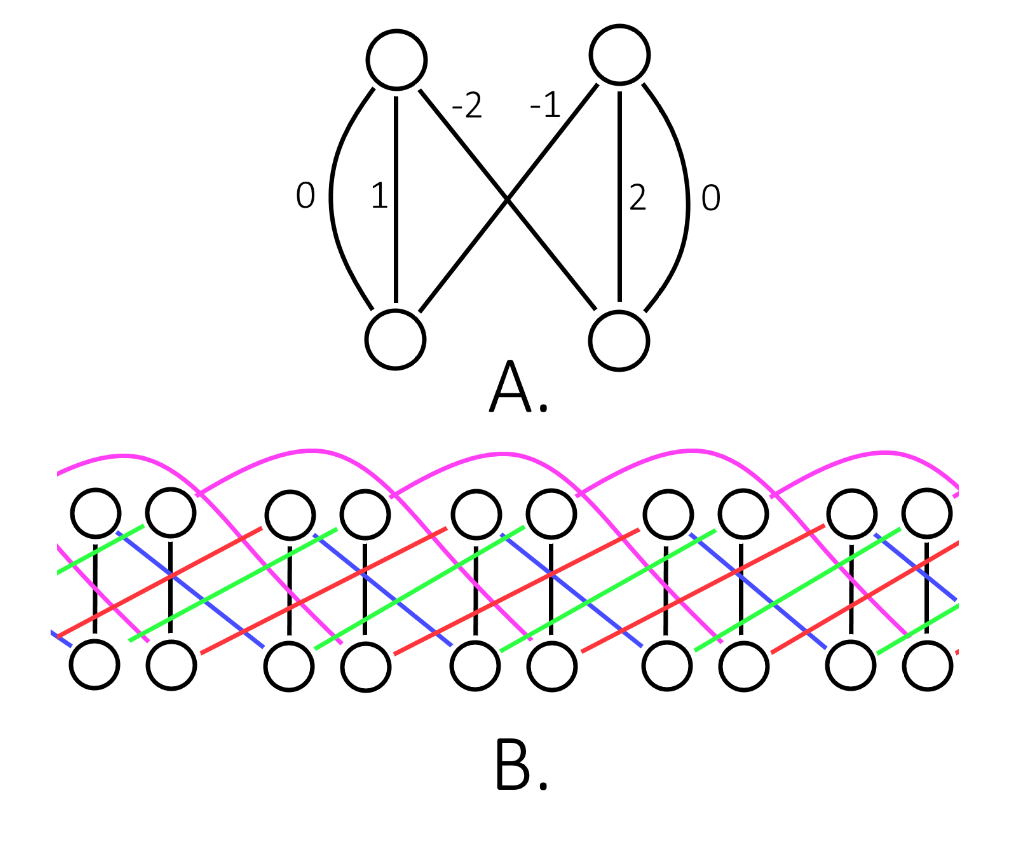
\includegraphics[scale=0.5]{Fig_7.png}
  \caption{ Граф полученный в результате работы алгоритма. A) В упрощённом представлении. B) В обычном представлении. }
  \label{stud:fig:7}
\end{figure}

 %=======================
\newpage

\section{Решение систем неравенств.}

Рассмотрим алгоритм 3 поиска решения системы неравенств с $e$ переменными:

\begin{itemize}
  \item В цикле по i от 1 до $e$:
  \begin{itemize}
    \item Находим все неравенства  вида $a x_i + b = 0$. Обозначим множество таких неравенств $I$.
    \item Выбираем число $v: v \neq -b/a \forall a x_i + b \in I$.
    \item Заменим во всех неравенствах $x_i$ на $v$ и выведем строку $x_i = v$.
  \end{itemize}
\end{itemize}

\textbf{Теорема.}

Вывод алгоритма 3 является решением системы неравенств.

\textbf{Доказательство.}

На $i$-той итерации работы алгоритма фиксируется значение $x_i$ таким образом, что ни одно неравенство не нарешается немедленно. Это возможно сделать, так как только неравенства вида $ax_i + b \neq 0$ могут немедленно нарушиться в результате фиксации значения $x_i$. Так как множество таких неравенств конечно, мы всегда можем найти число, удовлетворяющее им всем. Таким образом, в $e$-той итерации мы заменим последнюю переменную так, что ни одно неравенство не обратится в ноль. 

\qed

Так как алгоритм 3 всегда завершается, мы можем говорить о том, что если в результате поиска в общем виде не обнаружил цикла с длиной меньше или равной $t$, то можно получить граф с обхватом $t$ заменой неизвестных сдвигов на соответствующие решения системы неравенств в рассмариваемом графе с регулярными структурами.

%=======================
\newpage
\section{Метаграфы.}

Серьёзный недостаток алгоритма 2 в том, что в процессе его работы используется система неравенств, которая растёт экспоненциально от длины цикла. Для уменьшения этой системы неравенство можно использовать метаграфы \cite{metagraphs}.

\subsection{Определение.}

\textsl{Метаграф} ~--- это двудольный граф, дугам которого поставлены в соответствие двоичные матрицы. Из метаграфа можно получить граф таннера, если сопоставить каждой вершине набор из $K$ вершин, а каждой дуге ~--- набор дуг, построенный по соответствующей ей матрице размера $K \times K$. Такой процесс будем называть увеличением в $K$ раз. 

В качестве матриц в метаграфах будем использовать матрицы-\\циркулянты, образованных вектором, содержащим одну единицу и нули. Тогда одной дуге метаграфа будет соответствовать ровно $K$ дуг. Группа таких матриц размера $K$ изоморфна $Z_K$, поэтому можно ставить дугам в соответствие целые числа, подразумевая соответствующие матрицы. Далее будем говорить только о таких метаграфах.

На рис. \ref{stud:metagraph:1} изображён метаграф, с вершинами, помеченными числами, и результат увеличения его в 4 раза.

\begin{figure}[H]
  \centering
  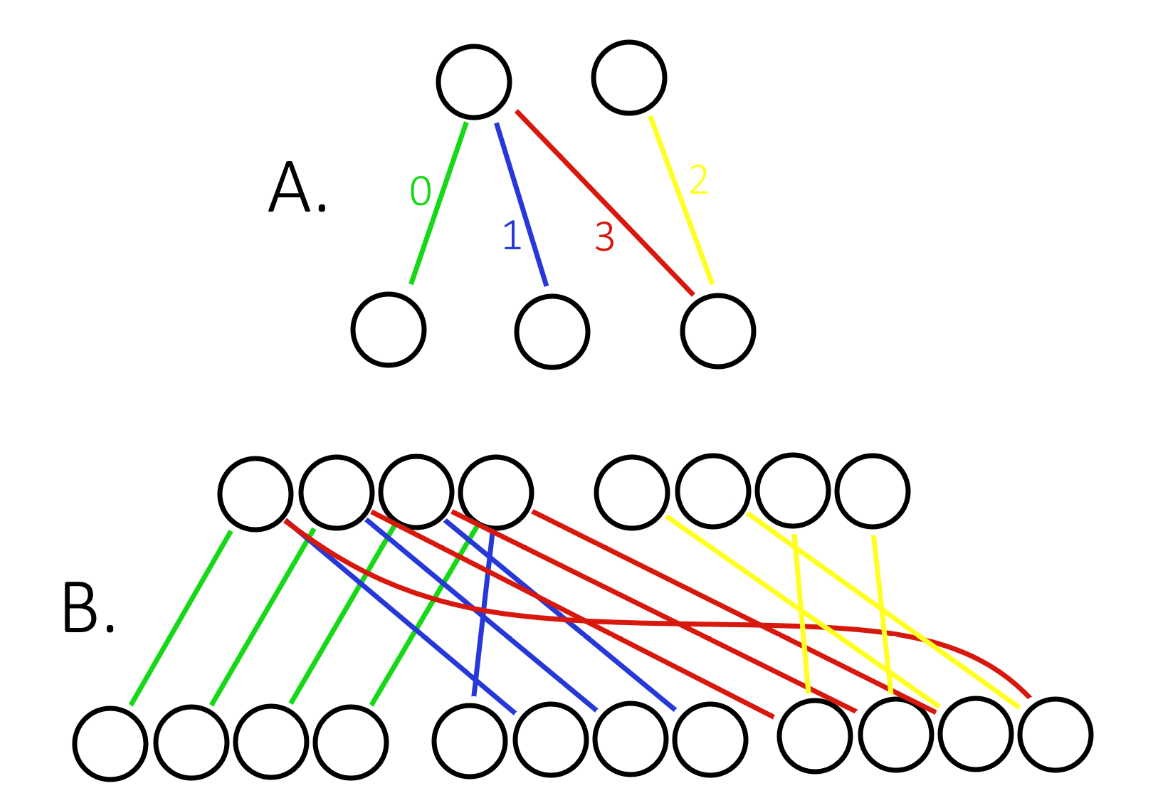
\includegraphics[scale=0.5]{Fig_8.png}
  \caption{ A) Метраграф. B) Результат увеличения метаграфа в 4 раза. }
  \label{stud:metagraph:1}
\end{figure}

\subsection{Поиск циклов.}

В работе \cite{metagraphs} показано, что цикл на метаграфе соответствует циклу на графе тогда и только тогда, когда сумма соответствующих дугам цикла чисел равна нулю по модулю $K$, причем числа дуг идущих от информационной вершины к проверочной должны быть взяты с обратным знаком.

Можно модифицировать алгоритм 1 таким образом, чтобы он искал циклы на метаграфах с регулярными структурами. Для этого будем использовать в качестве пометок не числа, а пары $(a, b)$, где $a$ ~--- относительный сдвиг, который ранее составлял всю метку, а $b$ ~--- накопленная сумма соответствующих дугам метаграфа меток. Пары $(a_1, b_2)$ и $(a_2, b_2)$ считаются одинаковыми, если $a_1 = a_2$ и $b_1 = b_2 \pmod K$. Когда к метке $(a, b)$ прибавляется сдвиг $s$ дуги, которой поставлено в соответствие число $c$, получается метка $(a + s, b + c \pmod K)$.

\begin{figure}[H]
  \centering
  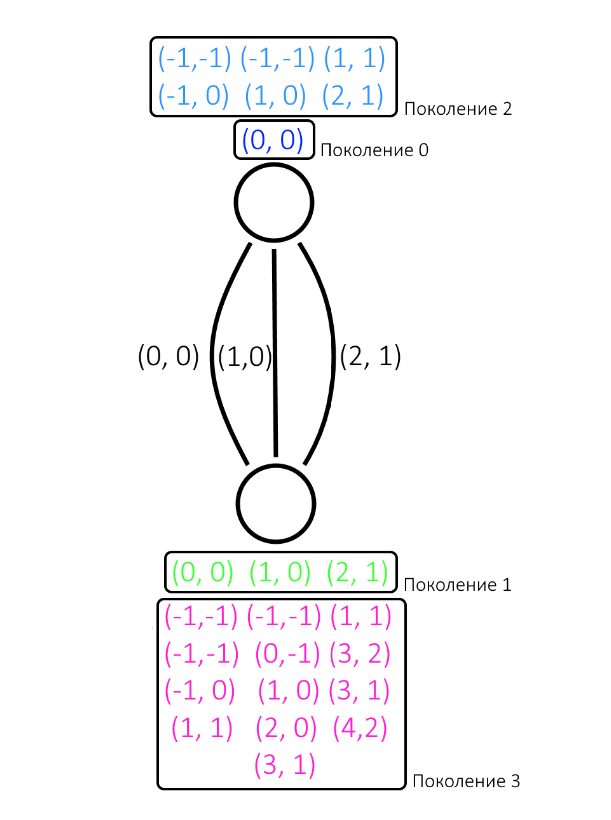
\includegraphics[scale=0.5]{Fig_9.png}
  \caption{ Работа алгоритма поиска циклов на метаграфе. }
  \label{stud:metagraph:2}
\end{figure}

На рис. \ref{stud:metagraph:2} изображена работа алгоритма поиска циклов на метаграфе. Найден цикл-шестёрка. Причём если отбросить числа, сопоставленные дугам в метаграфе и работать с ним, как с обычным двудольным графом, обхват уменьшится до 4.

\textbf{Замечание.}

Если алгоритм поиска циклов в графах с регулярной структурой обнаружил цикл в графе неизвестными сдвигами, то цикл найдётся и в метаграфе с такой структурой и неизвестными числами, поставленными в соответствие дугам.

\subsection{Использование в алгоритме построения графа с заданным обхватом}

Применим алгоритм 2, используя алгоритм поиска циклов на метаграфе, вместо обычного алгоритма поиска циклов, обозначив сдвиги дуг $x_1, ..., x_e$, а числа, поставленные им в соответствие ~--- $y_1, ..., y_e$. В результате получится система неравенств вида (\ref{stud:eqs:2}).

\begin{equation}
  \left\{
    \begin{array}{ll}
        \left[  
          \begin{array}{ll}
              a_1 x_1 + ... + a_e x_e \neq 0 \\
              a_1 y_1 + ... + a_e y_e \neq 0 \\
          \end{array}
        \right.\\
        ...\\
        \left[  
          \begin{array}{ll}
              b_1 x_1 + ... + b_e x_e \neq 0 \\
              b_1 y_1 + ... + b_e y_e \neq 0 \\
          \end{array}
        \right.\\
    \end{array}
  \right.
  \label{stud:eqs:2}
\end{equation}

Устройство системы неравенств позволяет заранее выбрать числа, поставленные в соответствие дугам и избавить от части неравенств ещё на этапе генерации системы. Хорошими вариантами значений для таких чисел являются числа из последовательности Сидона \cite{sidon}.

%=======================
\newpage
\addcontentsline{toc}{section}{Заключение}
\section*{Заключение}



%=======================
\newpage

\addcontentsline{toc}{section}{Литература}
\renewcommand{\refname}{\centering \textbf{Литература}}

\begin{thebibliography}{0}

\bibitem{johnson}
Johnson S.\,J.
Introducing Low-Density Parity-Check Codes.
~-- University of Newcastle, Australia, 2006.

\bibitem{bruteforce}
Гурский С.\,С., Могилевская Н.\,С.
Задача генерации проверочных матриц ldpc-кодов.
~-- Ростов н/Д : Материалы конференции СИТО, 2021.

\bibitem{permutations}
Gallager R.\,G. 
Low-density parity-check codes
~-- IRE Transactions on Information Theory, 1962.

\bibitem{metagraphs}
Арутюнов О.\,В.
Построение (m, n)-регулярных двудольных графов с наибольшим обхватом методом увеличения метаграфов.
~-- Ростов н/Д : Материалы конференции СИТО, 2021.

\bibitem{sidon}
Последовательности Сидона.


\end{thebibliography}

\end{document}
% ----------------------------------------------------------------


\lstset{ %
language=C++,                 % выбор языка для подсветки (здесь это С++)
basicstyle=\small\sffamily, % размер и начертание шрифта для подсветки кода
numbers=left,               % где поставить нумерацию строк (слева\справа)
numberstyle=\tiny,           % размер шрифта для номеров строк
stepnumber=1,                   % размер шага между двумя номерами строк
numbersep=5pt,                % как далеко отстоят номера строк от подсвечиваемого кода
backgroundcolor=\color{white}, % цвет фона подсветки - используем \usepackage{color}
showspaces=false,            % показывать или нет пробелы специальными отступами
showstringspaces=false,      % показывать или нет пробелы в строках
showtabs=false,             % показывать или нет табуляцию в строках
frame=single,              % рисовать рамку вокруг кода
tabsize=2,                 % размер табуляции по умолчанию равен 2 пробелам
captionpos=t,              % позиция заголовка вверху [t] или внизу [b]
breaklines=true,           % автоматически переносить строки (да\нет)
breakatwhitespace=false, % переносить строки только если есть пробел
escapeinside={\%*}{*)}   % если нужно добавить комментарии в коде
extendedchars=true,
commentstyle=\color{mygreen},    % comment style
stringstyle=\bf,
commentstyle=\ttfamily\itshape,
keepspaces=true % пробелы между русскими буквами
aboveskip=3mm,
belowskip=3mm

}


\renewcommand\NAT@bibsetnum[1]{\settowidth\labelwidth{\@biblabel{#1}}%
   \setlength{\leftmargin}{\bibindent}\addtolength{\leftmargin}{\dimexpr\labelwidth+\labelsep\relax}%
   \setlength{\itemindent}{-\bibindent+\fivecharsapprox}%
   \setlength{\listparindent}{\itemindent}
\setlength{\itemsep}{\bibsep}\setlength{\parsep}{\z@}%
   \ifNAT@openbib
     \addtolength{\leftmargin}{\bibindent}%
     \setlength{\itemindent}{-\bibindent}%
     \setlength{\listparindent}{\itemindent}%
     \setlength{\parsep}{0pt}%
   \fi
}
\renewcommand{\thesection}{\arabic{section}.}
\renewcommand{\thesubsection}{\arabic{section}.\arabic{subsection}.}
